%% Supplementary material for the Artemis II seismo-acoustic paper.
%% Compile:  latexmk -pdf Artemis2supplement.tex
\documentclass[11pt]{article}
\usepackage[margin=2.2cm]{geometry}
\usepackage{graphicx}
\usepackage{siunitx}
\usepackage[font=small]{caption}
\graphicspath{{figures/}}
\renewcommand{\thefigure}{S\arabic{figure}}
\setlength{\parindent}{0pt}

\title{Supplementary material for\\ ``Seismo-acoustic observations of the Artemis~II launch:
  Insights from a dense ground-based network at Kennedy Space Center''}
\author{Glenn Thompson, Paul Bremner, Han Byul Woo, Sue Bilek}
\date{}

\begin{document}
\maketitle

Figures S1--S12 support the main text. They were produced by the notebooks in
\texttt{09\_artemis2\_paper} (numbers in brackets).

\begin{figure}[p]
  \centering
  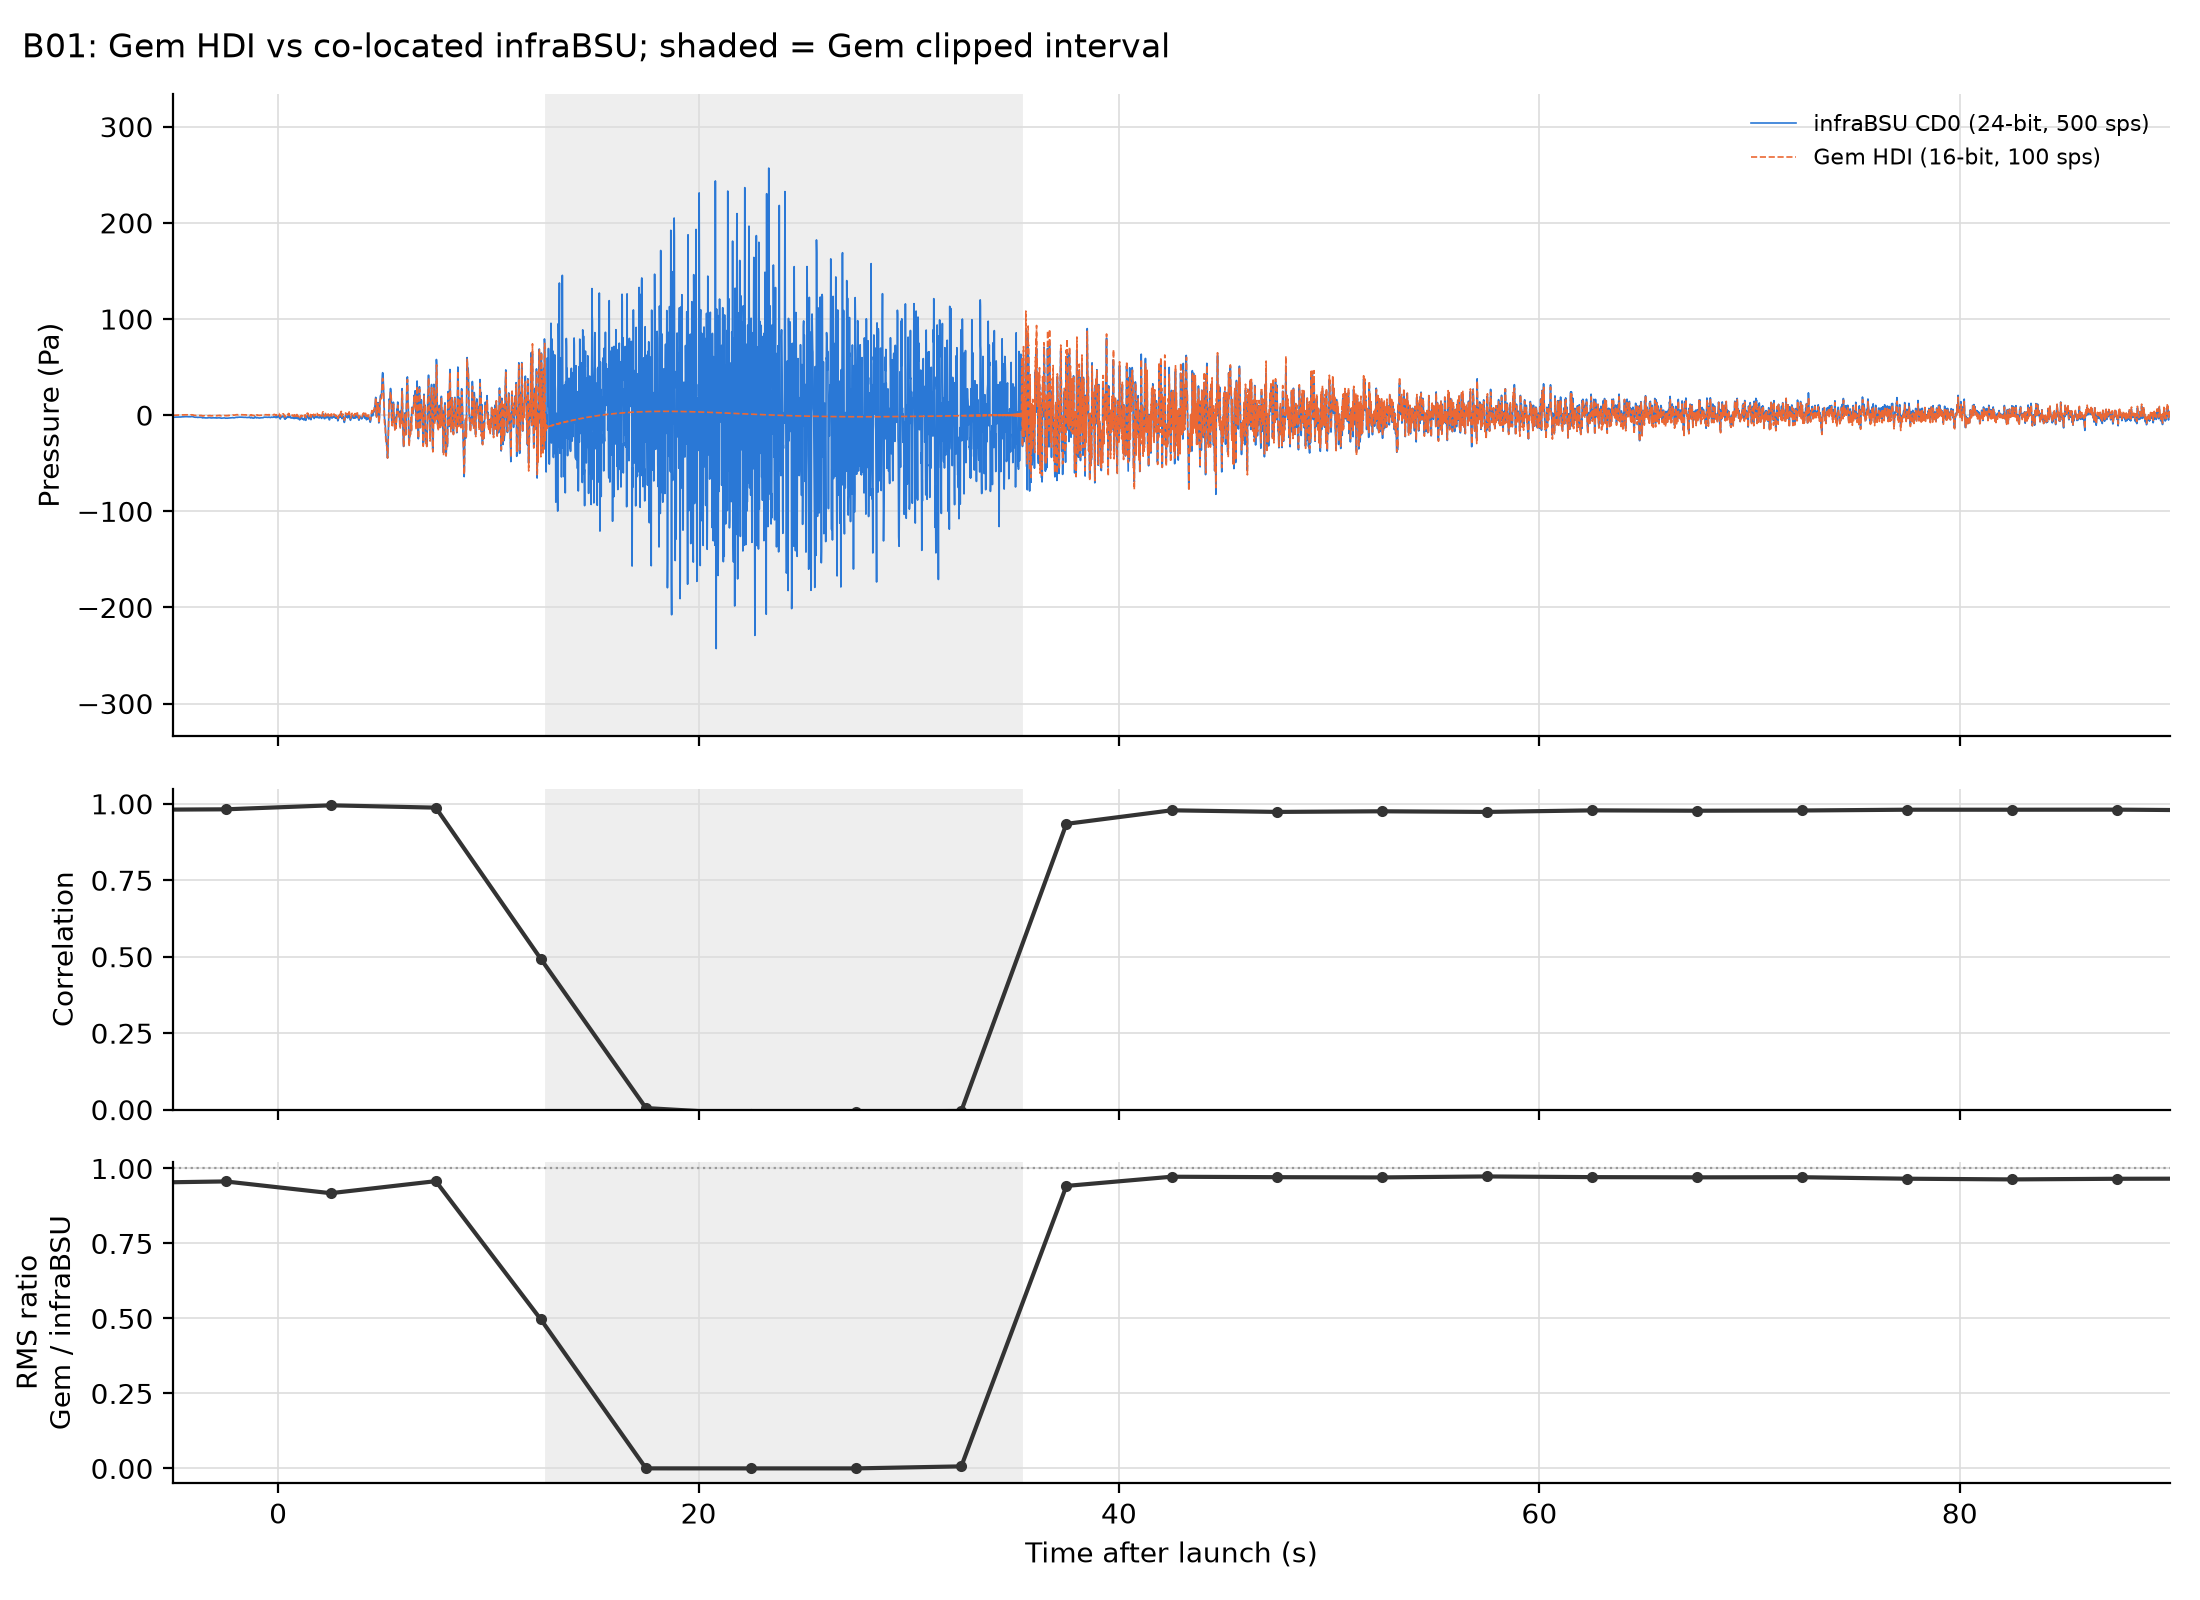
\includegraphics[width=\textwidth]{clipping_validation_B01}
  \caption{Validation of the Gem overflow intervals at B01 [20]. Top: corrected
    pressure from the infraBSU (DD0, 24-bit, 500~samples~s$^{-1}$) and the
    co-located Gem (HDI, 16-bit, 100~samples~s$^{-1}$); shaded: the Gem's
    overflow interval. Middle and bottom: correlation and RMS ratio of the two
    records in 5-s windows (1--20~Hz). Outside the interval the Gem tracks the
    infraBSU (correlation 0.99, ratio 0.96). The Gem is shown after the
    overflow repair (Section~3.3 of the main text): inside the interval its
    samples are bridged by a straight line and carry no signal.}
\end{figure}

\begin{figure}[p]
  \centering
  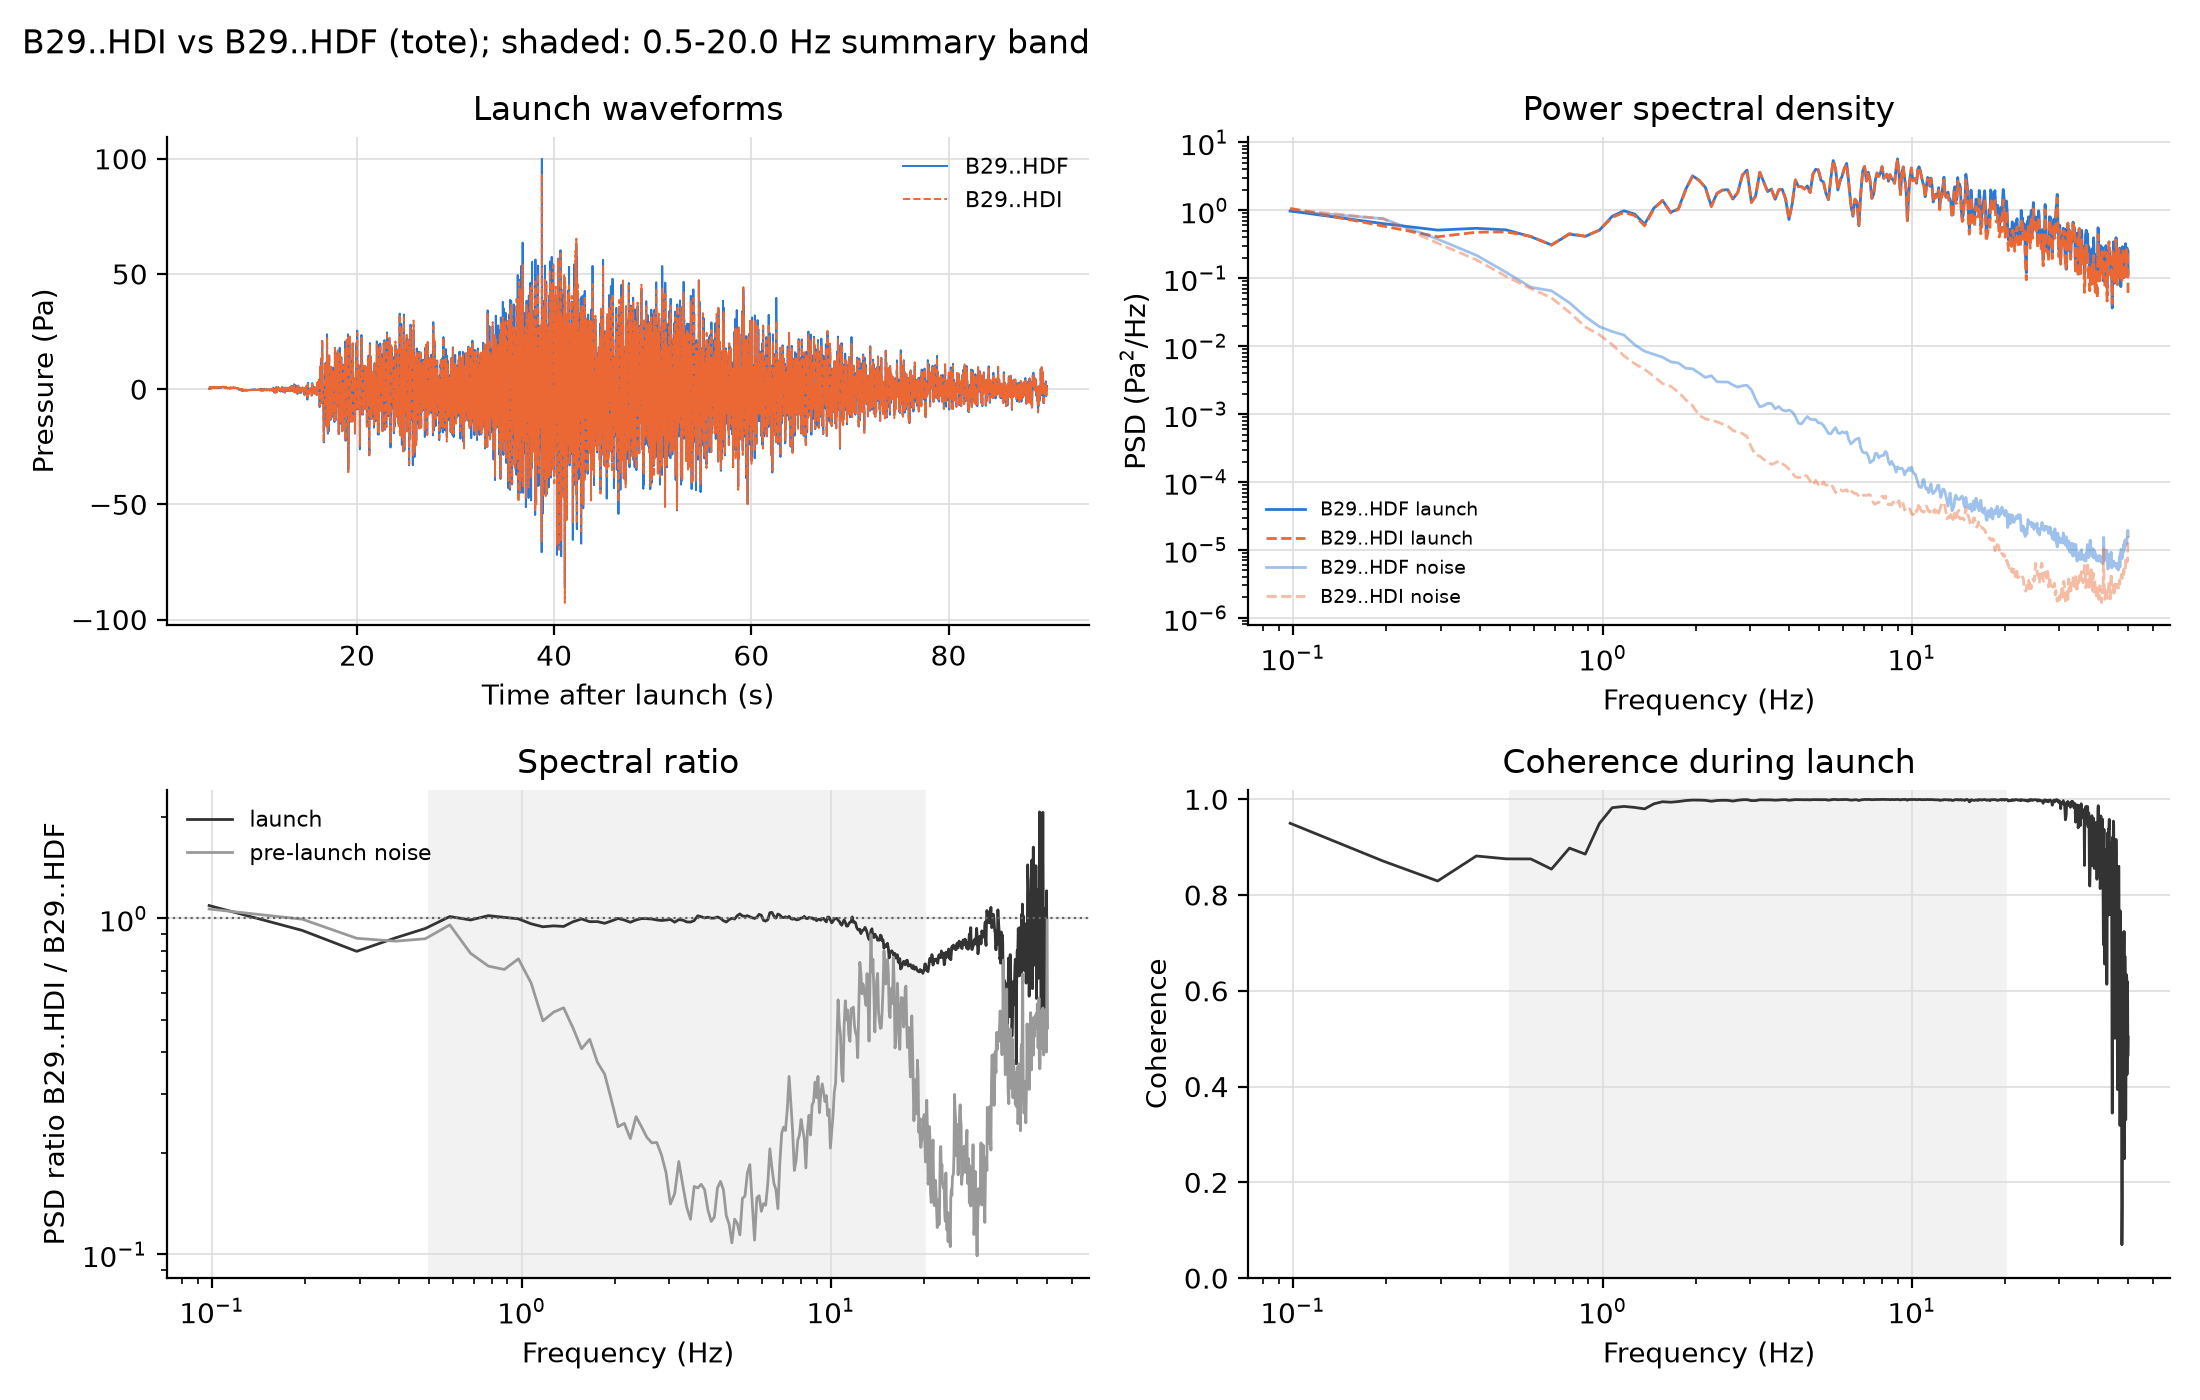
\includegraphics[width=\textwidth]{enclosure_B29__HDF_vs_B29__HDI}
  \caption{Tote (HDI) versus free-field (HDF) Gem at B29 [30]: launch
    waveforms, power spectral densities during the launch and in pre-launch
    noise, spectral ratio, and coherence during the launch. Shaded: the
    0.5--20~Hz band used for summary values.}
\end{figure}

\begin{figure}[p]
  \centering
  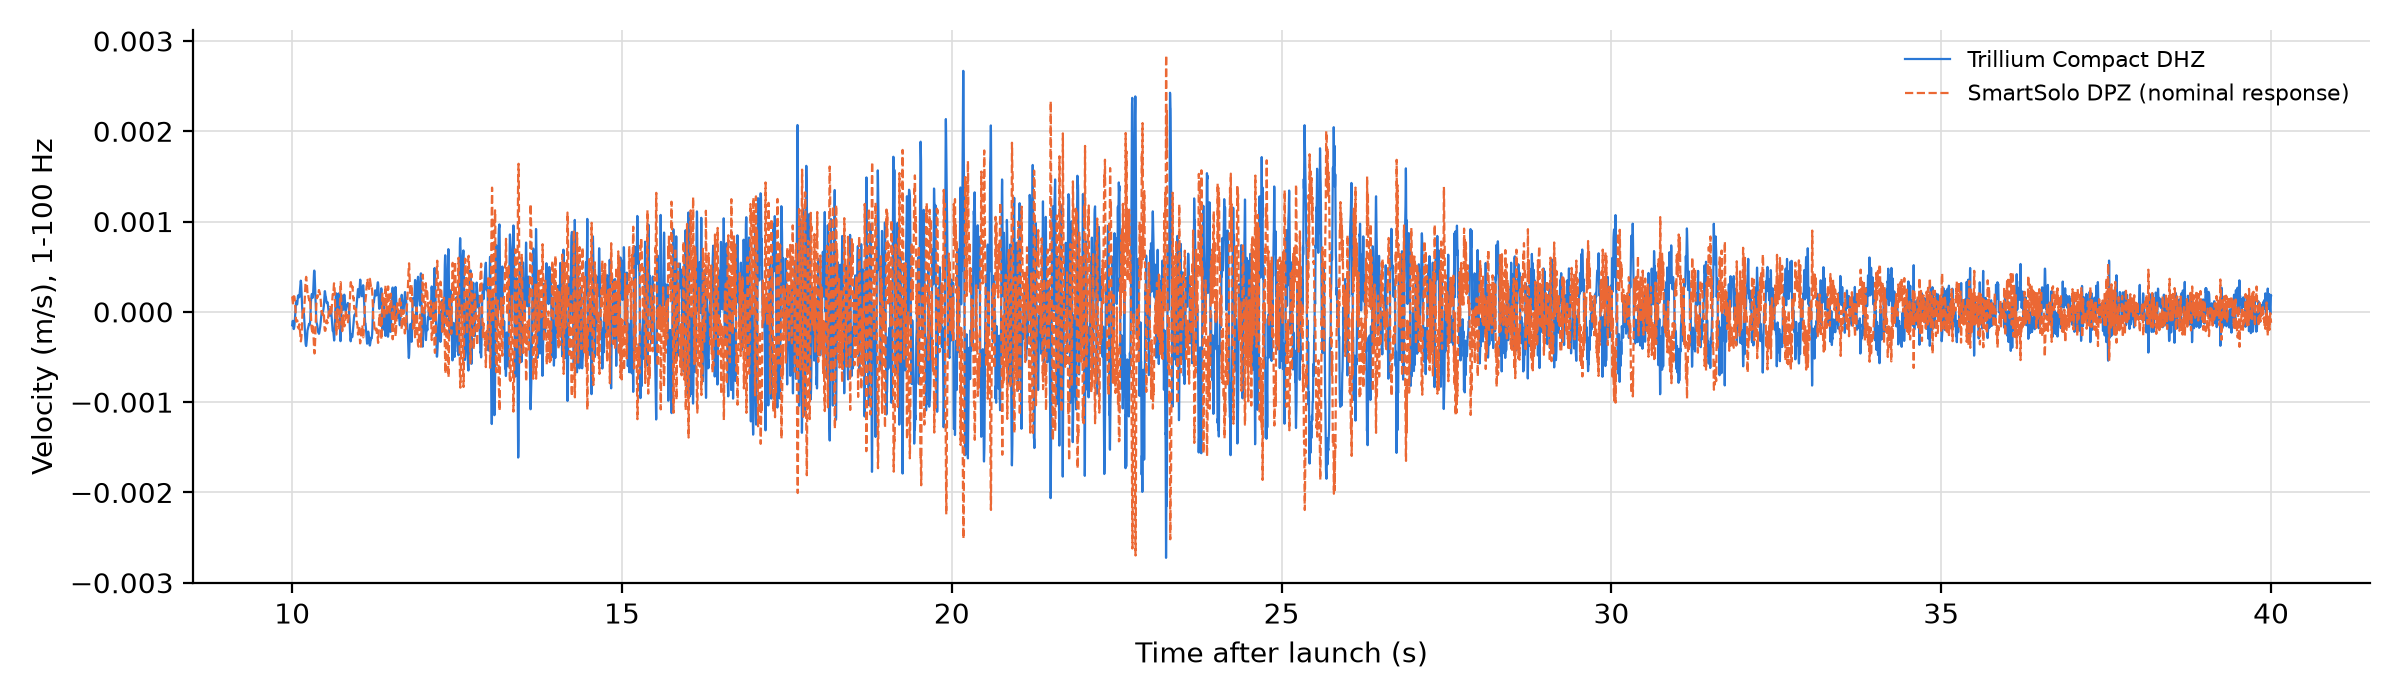
\includegraphics[width=\textwidth]{smartsolo_vs_trillium_B01_waveforms}
  \caption{Vertical velocity at B01 from the Trillium Compact (DHZ) and the
    SmartSolo node (DPZ) after removal of the nominal 5~Hz geophone response,
    1--100~Hz [45]. Peak velocities agree within 4\%. The SmartSolo trace is
    shown as recorded (reversed polarity).}
\end{figure}

\begin{figure}[p]
  \centering
  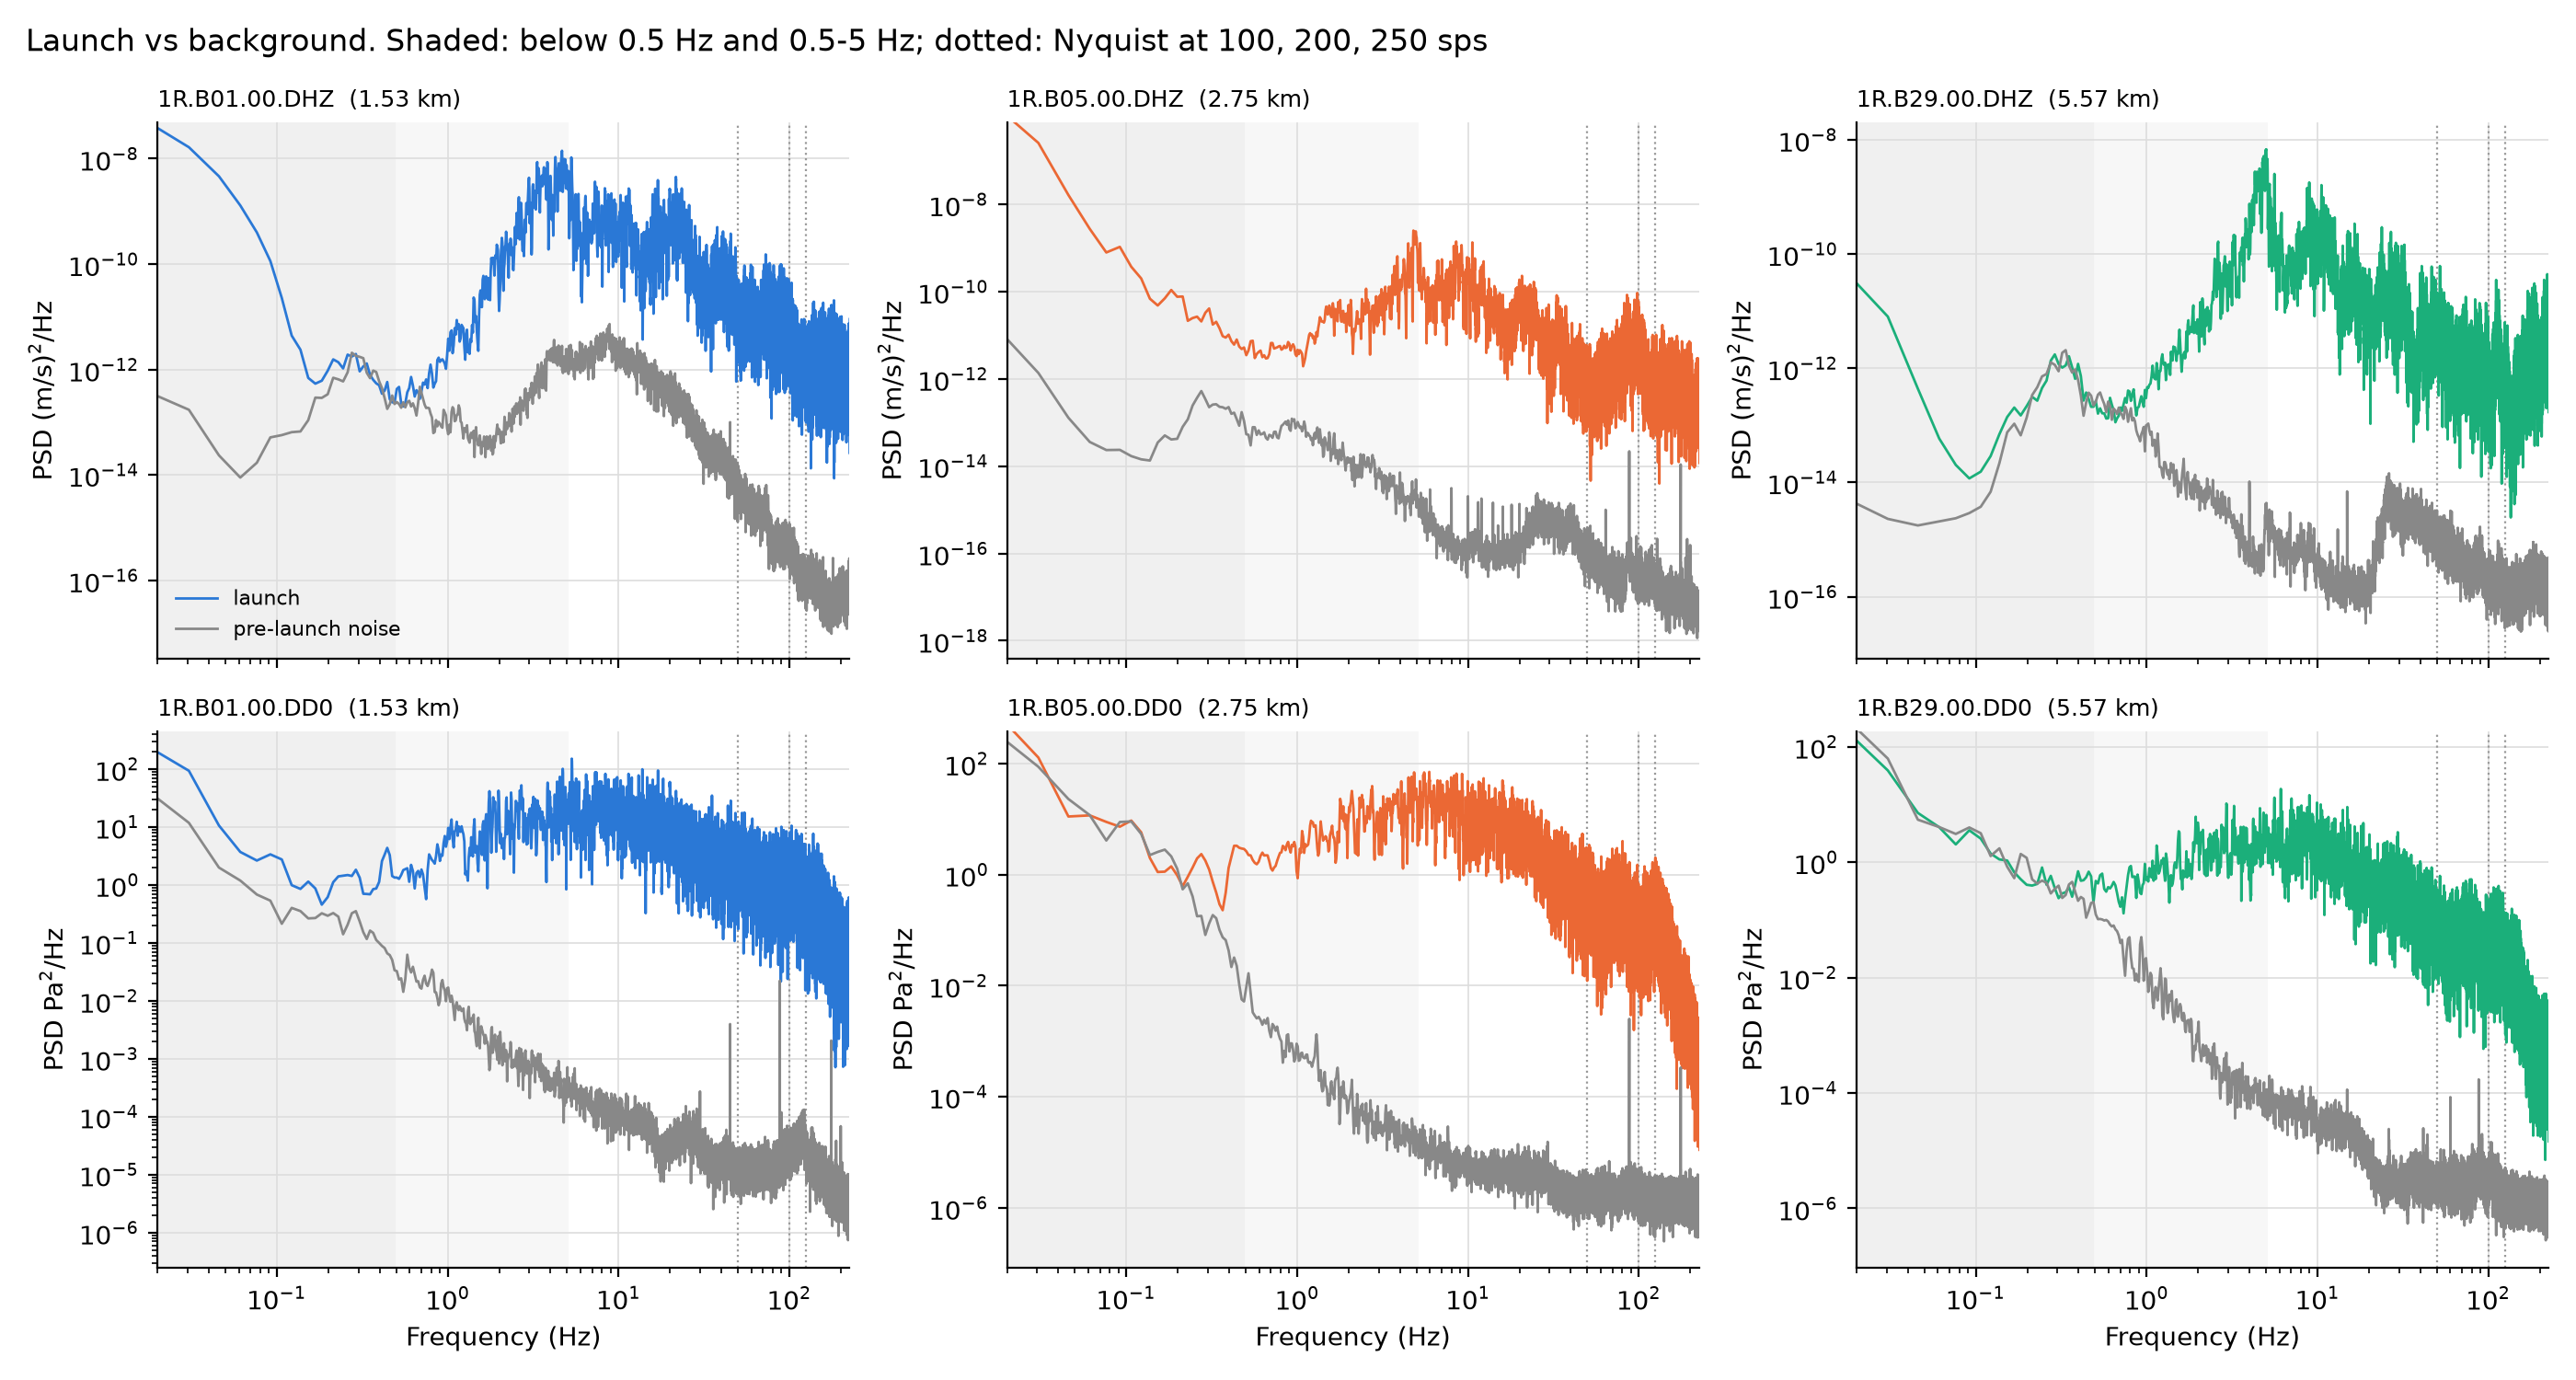
\includegraphics[width=\textwidth]{bandwidth_psd}
  \caption{Power spectral density during the launch and in pre-launch noise
    for vertical velocity (top) and pressure (bottom) at B01, B05 and B29
    [45]. Shaded: below 0.5~Hz and 0.5--5~Hz; dotted: Nyquist frequencies of
    100, 200 and 250~samples~s$^{-1}$.}
\end{figure}

\begin{figure}[p]
  \centering
  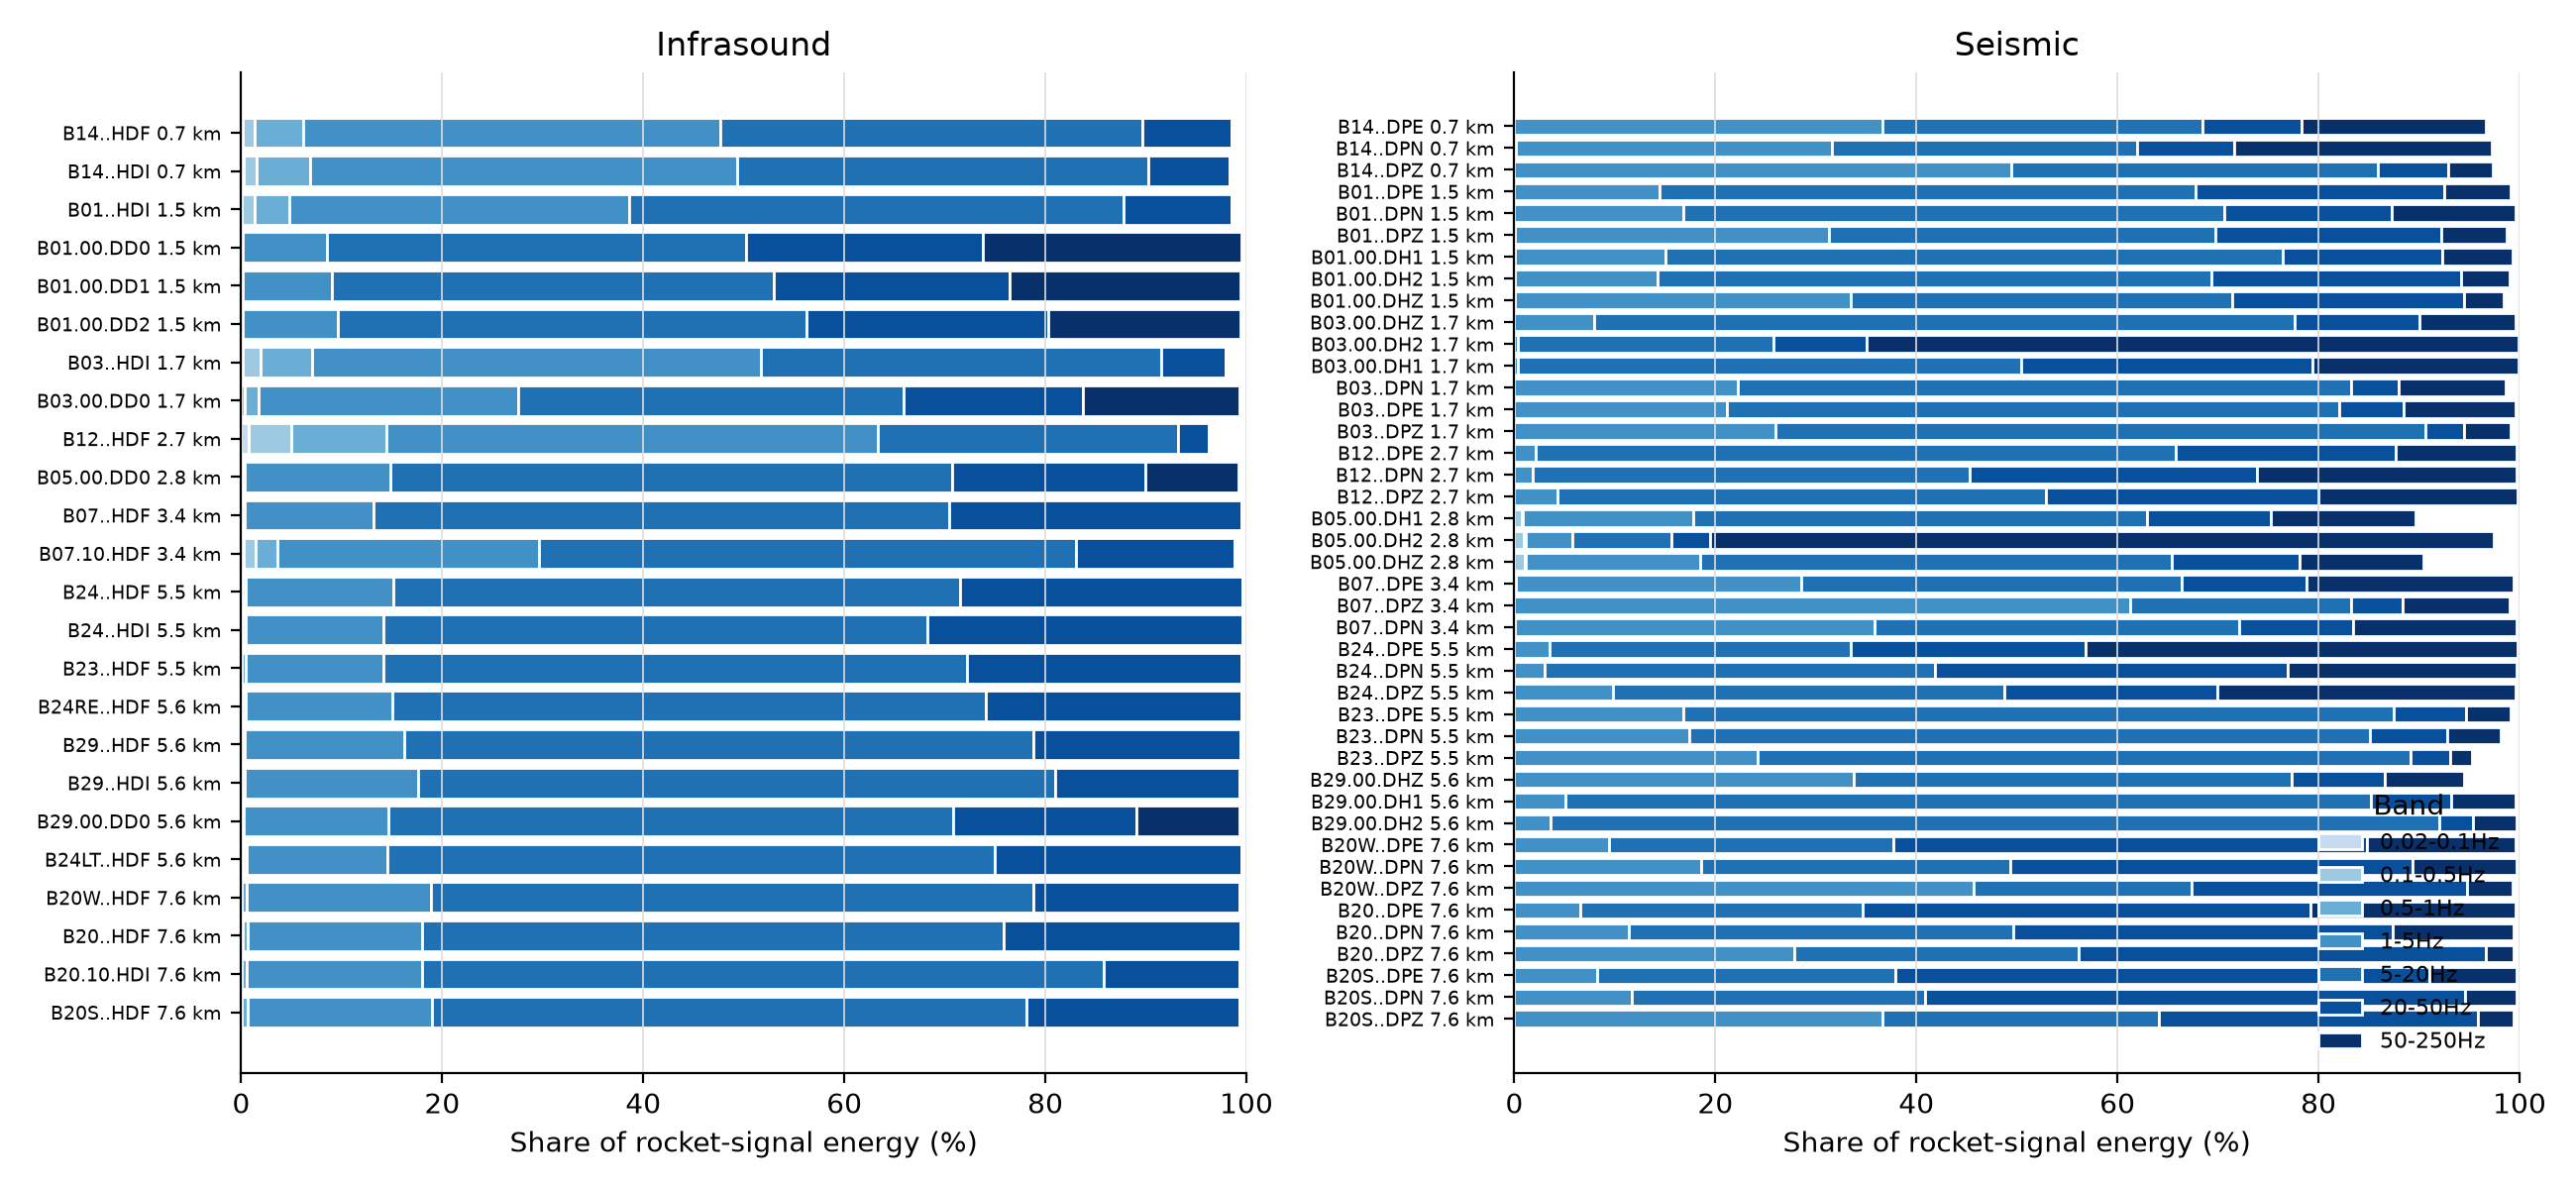
\includegraphics[width=\textwidth]{snr_band_energy}
  \caption{Share of rocket-signal energy (launch minus noise PSD) in frequency
    bands for every pressure (left) and velocity (right) channel, sorted by
    distance [42]. Gem spectra end at 45~Hz and SmartSolo spectra are
    meaningful only above 1~Hz.}
\end{figure}

\begin{figure}[p]
  \centering
  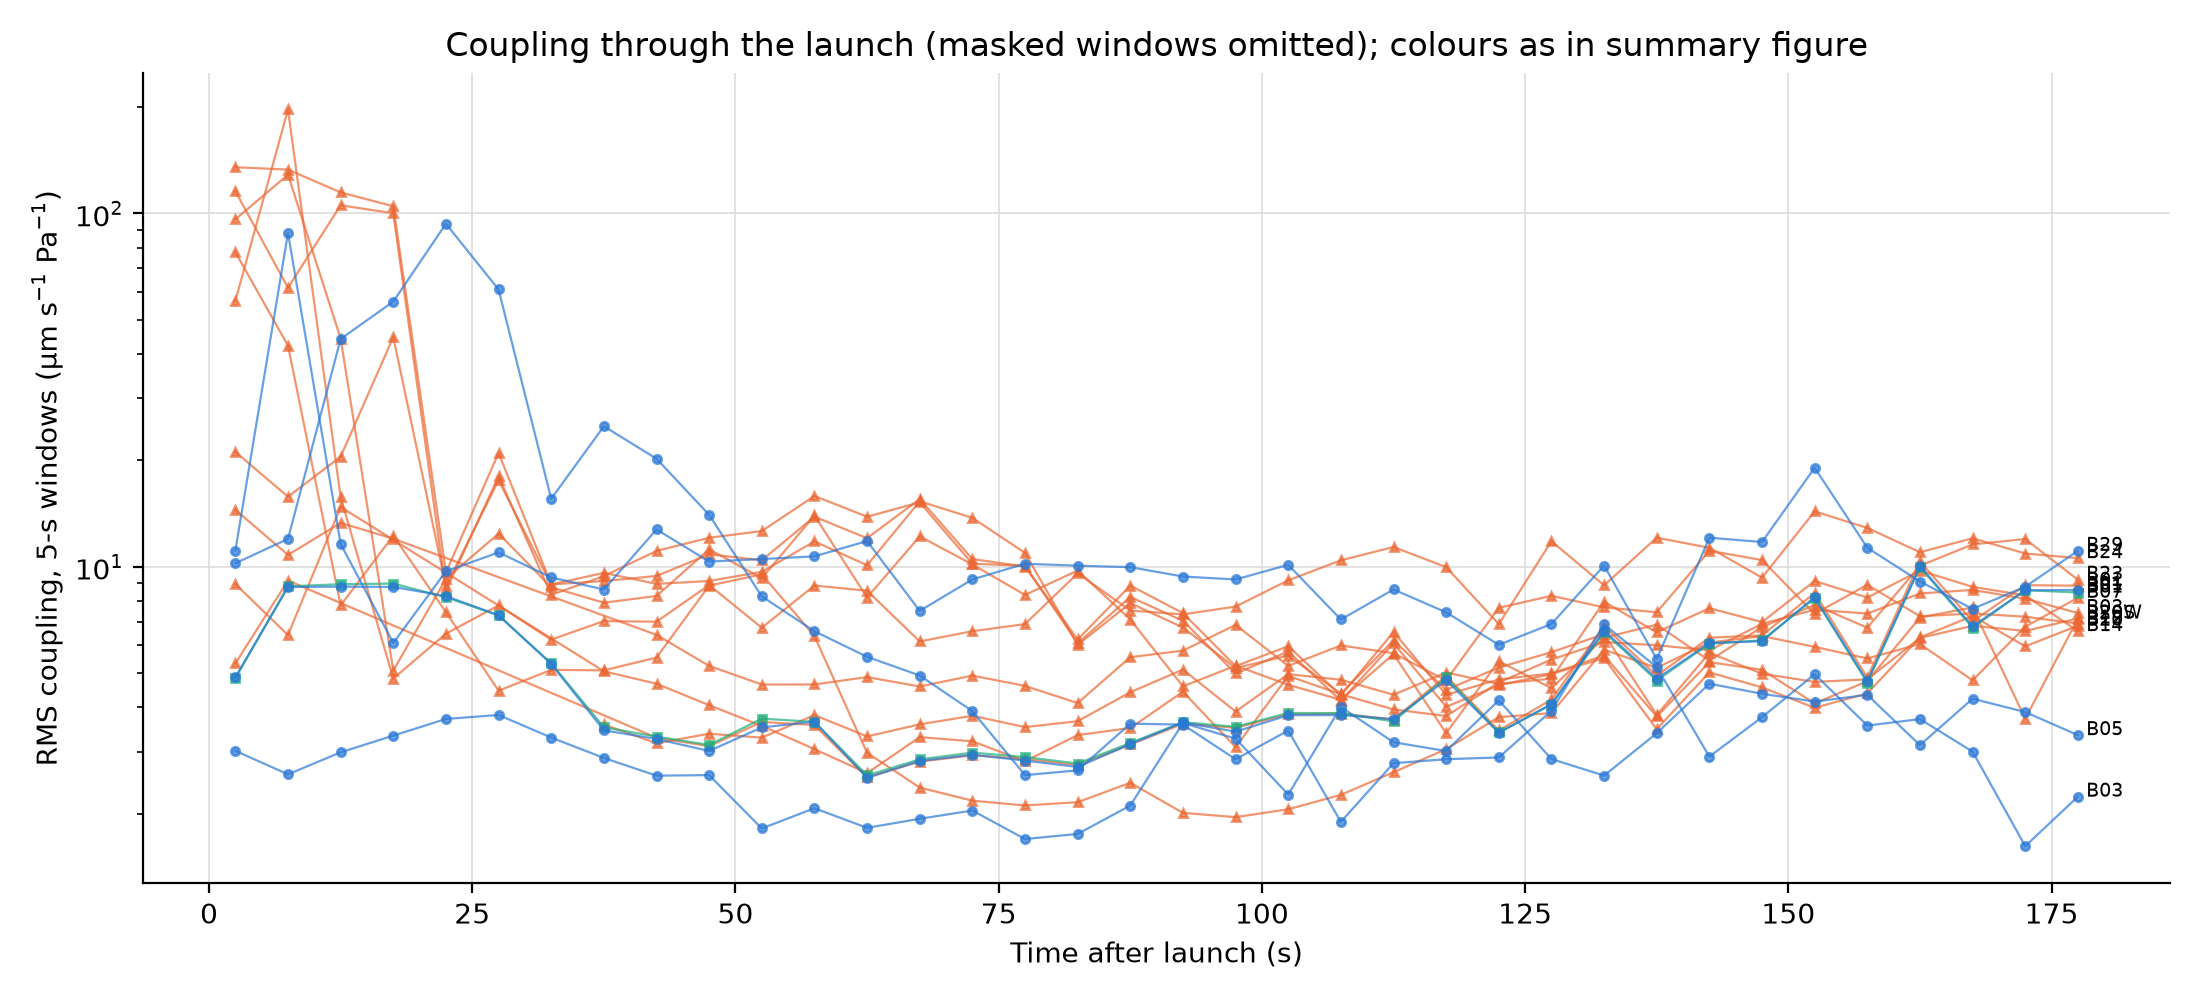
\includegraphics[width=\textwidth]{coupling_vs_time}
  \caption{RMS ratio of vertical velocity to pressure (1--40~Hz) in 5-s
    windows through the launch for each co-located pair [50]. Windows
    overlapping Gem overflow are omitted. At the distant B20 sites the ratio
    is high before the air wave arrives, because ground motion from the pad
    arrives first.}
\end{figure}

\begin{figure}[p]
  \centering
  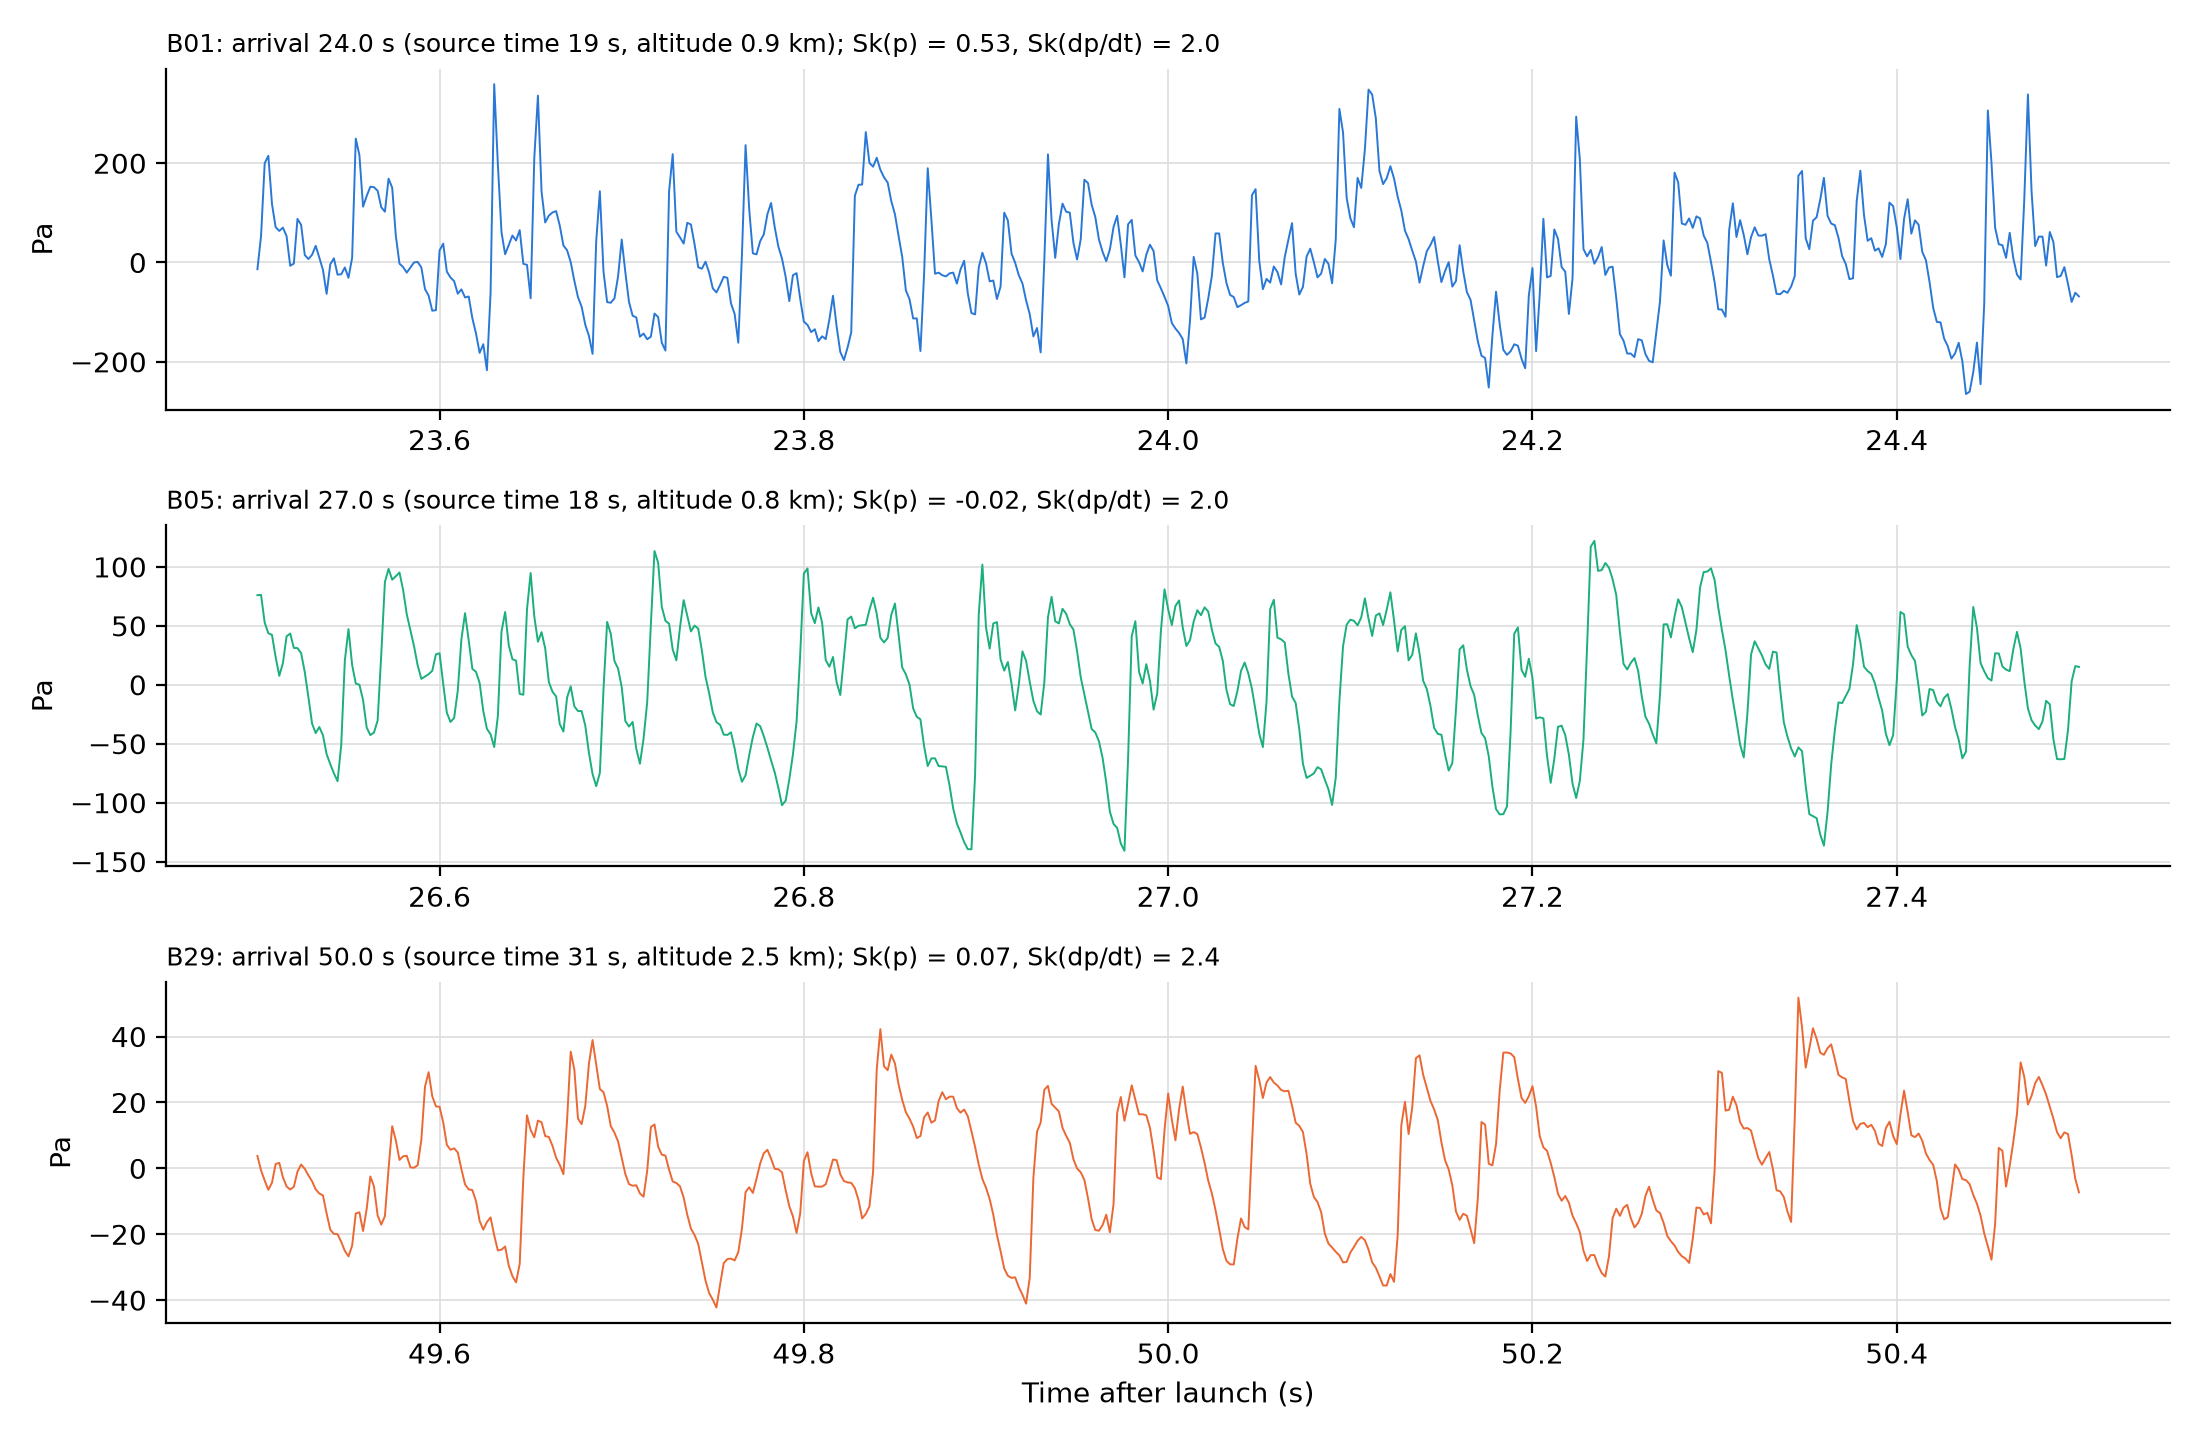
\includegraphics[width=\textwidth]{crackle_waveforms}
  \caption{One-second excerpts with the largest derivative skewness at B01,
    B05 and B29 for source times 10--45~s [55], showing steep pressure rises
    followed by slower decays.}
\end{figure}

\begin{figure}[p]
  \centering
  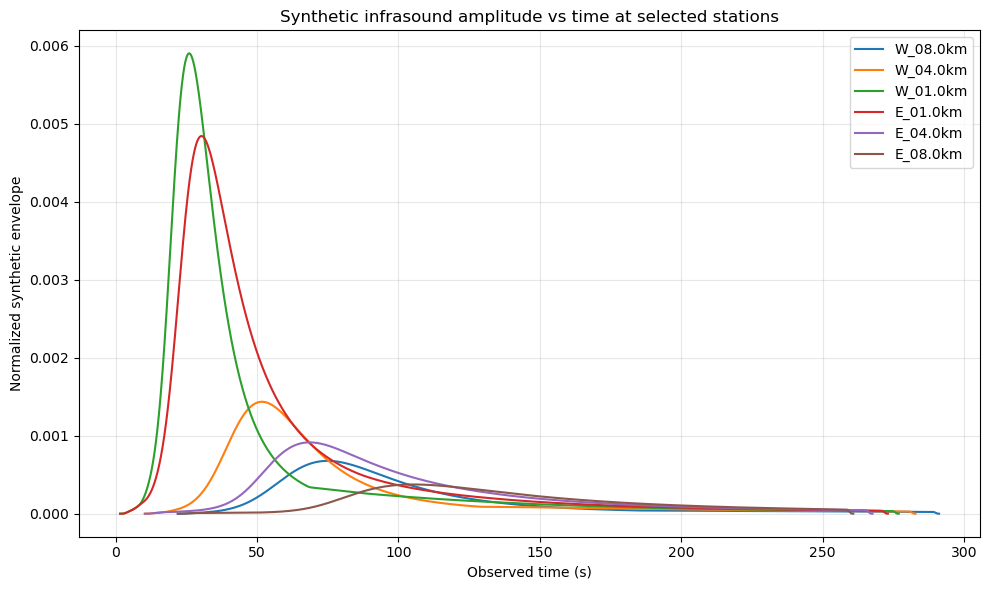
\includegraphics[width=\textwidth]{synthetic_envelopes}
  \caption{Synthetic infrasound envelopes at selected west (W) and east (E)
    virtual stations as a function of observed time [35], for the originally
    assumed directivity ($\phi_0 = 30^{\circ}$, $\sigma = 20^{\circ}$). At a
    given distance, west stations peak earlier and with higher amplitude than
    east stations.}
\end{figure}

\begin{figure}[p]
  \centering
  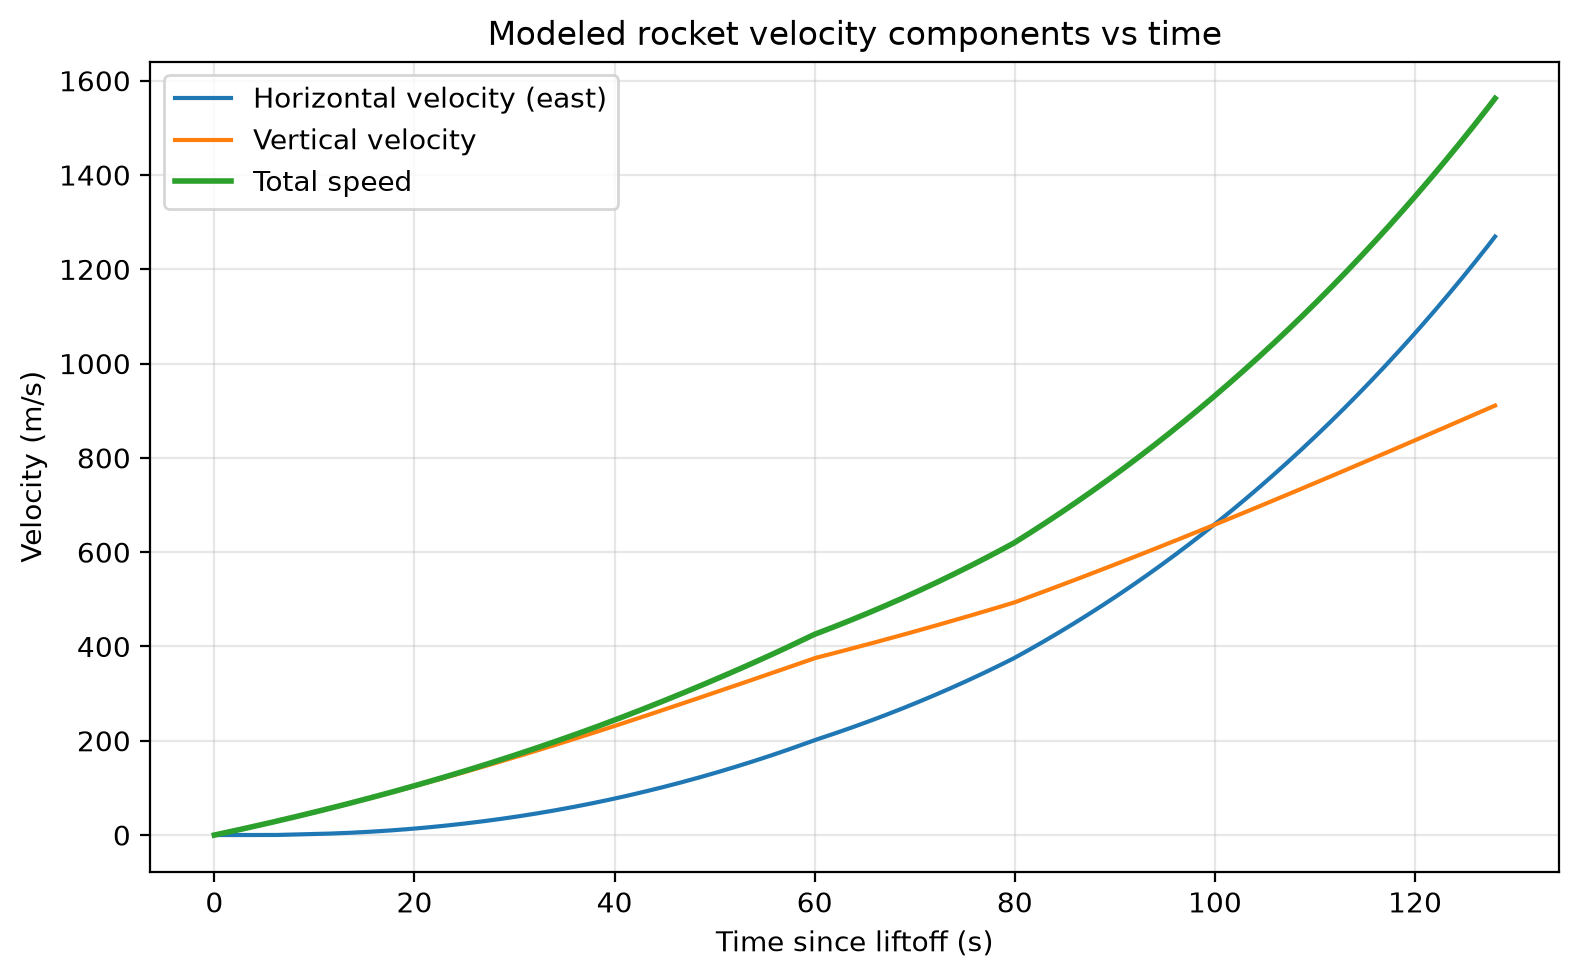
\includegraphics[width=0.85\textwidth]{velocity_vs_time}
  \caption{Modeled rocket velocity components and total speed versus time
    since liftoff [35].}
\end{figure}

\begin{figure}[p]
  \centering
  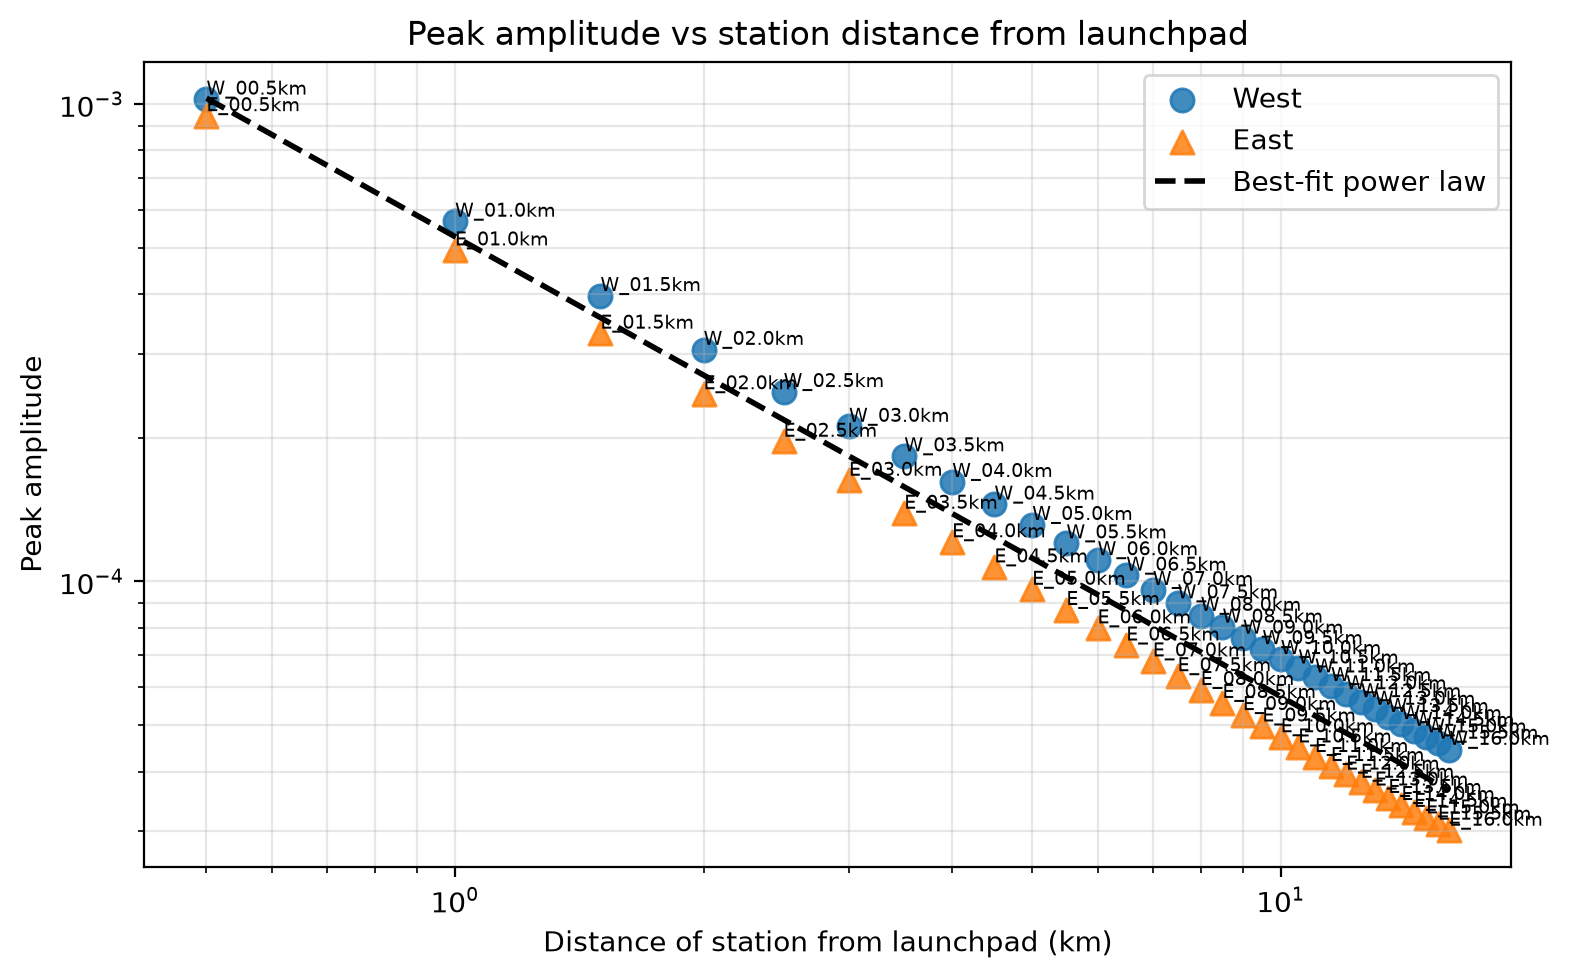
\includegraphics[width=0.8\textwidth]{synthetic_amplitude_vs_distance}
  \caption{Synthetic peak amplitude versus distance on idealized west (circles)
    and east (triangles) station lines for the originally assumed directivity
    (30$^{\circ}$, 20$^{\circ}$), with the best-fit power law (exponent
    $-0.96$) [35].}
\end{figure}

\begin{figure}[p]
  \centering
  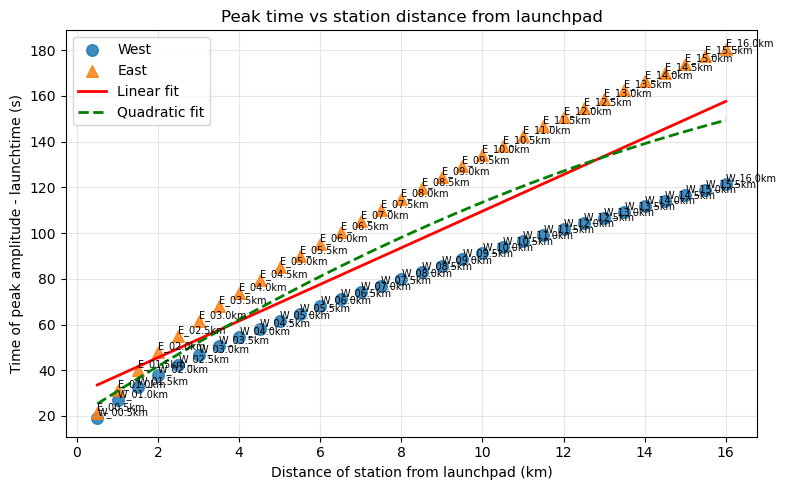
\includegraphics[width=0.8\textwidth]{synthetic_peaktime_vs_distance}
  \caption{Synthetic peak arrival time versus distance on the idealized lines
    for the originally assumed directivity [35]. Red: linear fit
    $t = 29.6 + 8.0\,r$~s ($r$ in km, apparent speed 125~m~s$^{-1}$); green
    dashed: quadratic fit.}
\end{figure}

\begin{figure}[p]
  \centering
  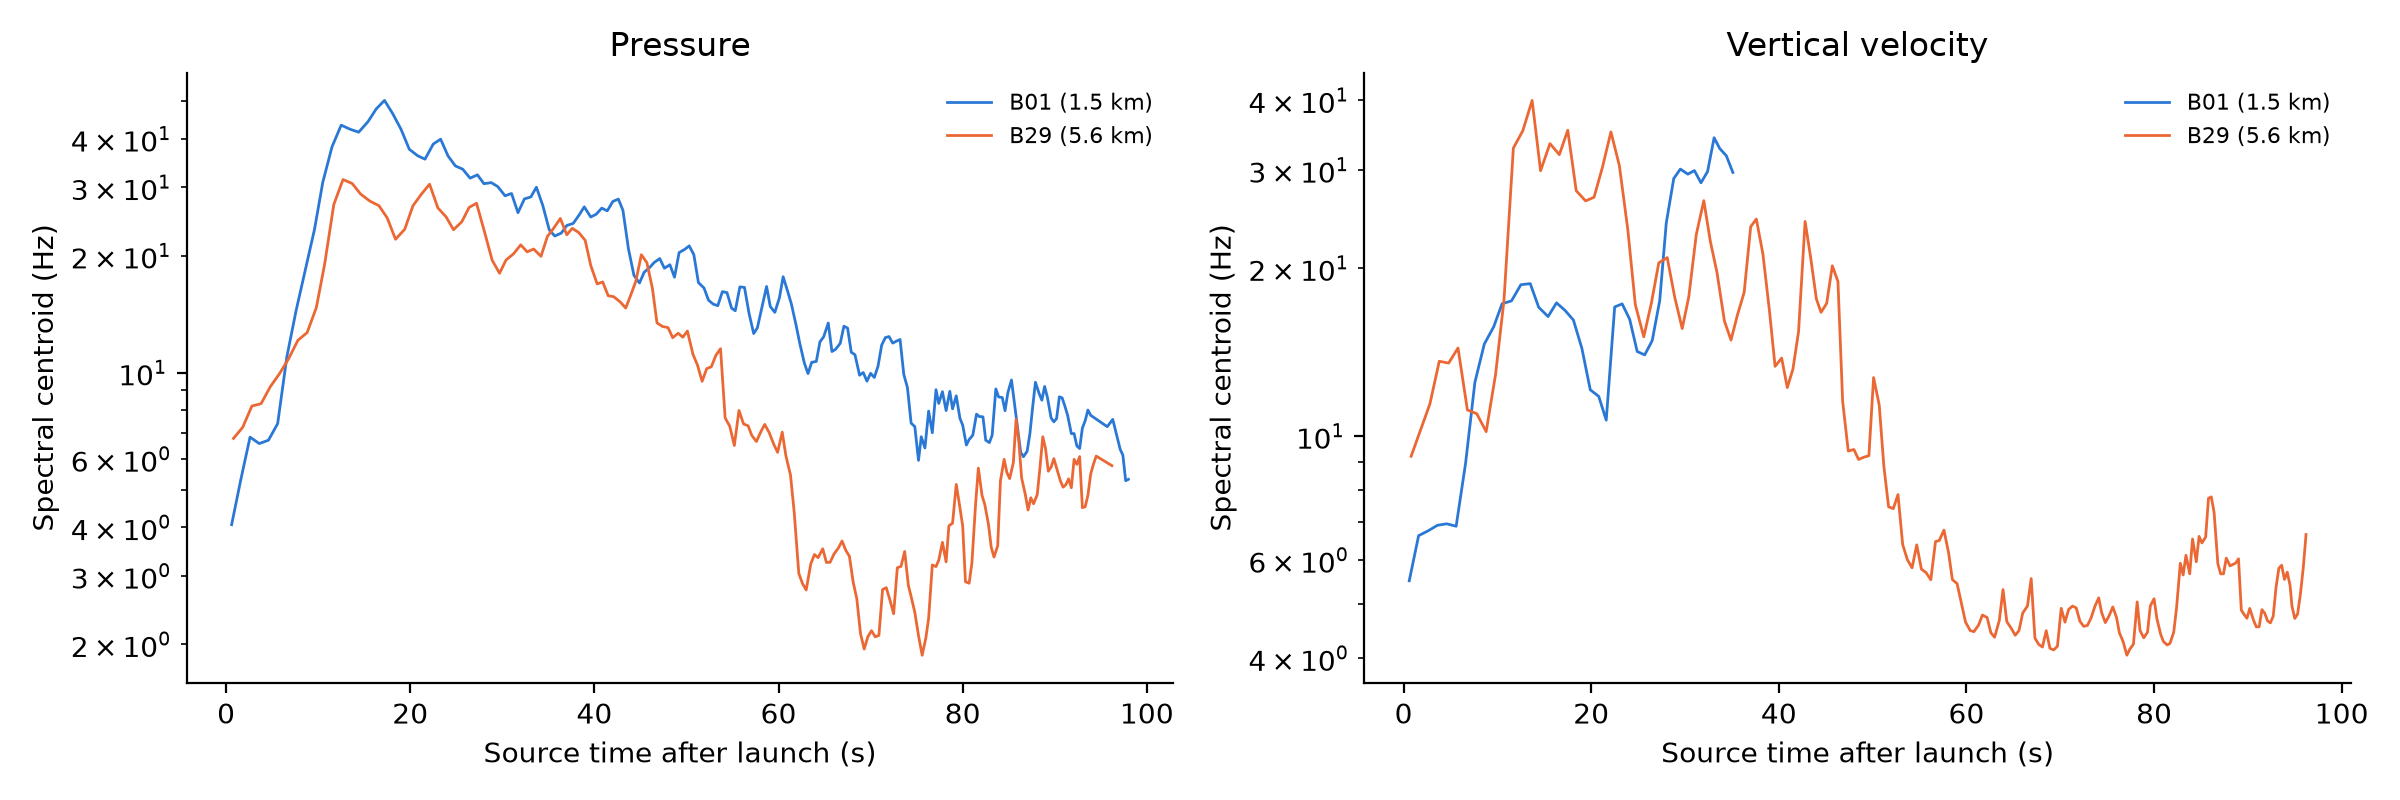
\includegraphics[width=\textwidth]{near_far_centroid}
  \caption{Spectral centroid of pressure (left) and vertical velocity (right)
    in 4-s windows at B01 and B29, plotted at the source time of emission
    [48]. Windows less than ten times the pre-launch noise are omitted, which
    ends the B01 seismic curve at $\sim$35~s.}
\end{figure}

\end{document}
